\section{Results}

\subsection{Evaluation questions}

The benchmark test suite was executed on seven LLMs listed below. 
\begin{itemize}
    \item \texttt{anthropic/claude-opus-4.6}
    \item \texttt{anthropic/claude-sonnet-4.6}
    \item \texttt{openai/gpt-5.4}
    \item \texttt{openai/gpt-5.4-mini}
    \item \texttt{deepseek/deepseek-v3.2}
    \item \texttt{google/gemini-3-flash-preview}
    \item \texttt{x-ai/grok-4-fast}
\end{itemize}

Taken together, the results are designed to answer the following questions:

\begin{enumerate}
    \item \textbf{Reliability.} Do the evaluated models complete the tasks without erroring? Are any failures concentrated on a particular model or task class?
    \item \textbf{Task difficulty.} Which benchmark tasks are intrinsically hard?
    \item \textbf{Resource usage.} How much context and how many output tokens does each model consume on average?
    \item \textbf{Token efficiency.} Does the duration scale predictably with token volume? Or do some models exhibit anomalous latency?
    \item \textbf{Cost.} What is the monetary cost per completed run? How large is the spread between providers?
    \item \textbf{Per-task model comparison.} Are the slowdowns concentrated on a particular subset of tasks?
    \item \textbf{Agent behaviour.} Do the models exhibit tool usage patterns that can explain their differences in cost and duration?
\end{enumerate}

\subsection{Task completion}

\begin{table}[htb]
    \centering
    \caption{Task completion by model}
    \label{tab:task-completion}
    \begin{tabular}{lr}
        \hline
        \textbf{Metric} & \textbf{Value} \\
        \hline
        Jobs (model $\times$ task pairs) & 119 \\
        Completed (latest run succeeded) & 117 \\
        Failed (latest run errored) & 2 \\
        Pending (not yet executed) & 0 \\
        Recorded runs (individual executions) & 355 \\
        \hline
    \end{tabular}
\end{table}

As seen in Table \ref{tab:task-completion}, the task completion rate is $117/119 = 98.3\%$.
Two executions are missing because one model abandoned the image tasks after its first failure.
Both of the two failed jobs were produced by \texttt{deepseek-v3.2} on the image tasks.
This is because this particular model does not support image capabilities.
This answers question~(1): the selected models can adequately complete the tasks as long as they are equipped with the multimodal capabilities afforded.

\begin{figure}[htb]
    \centering
    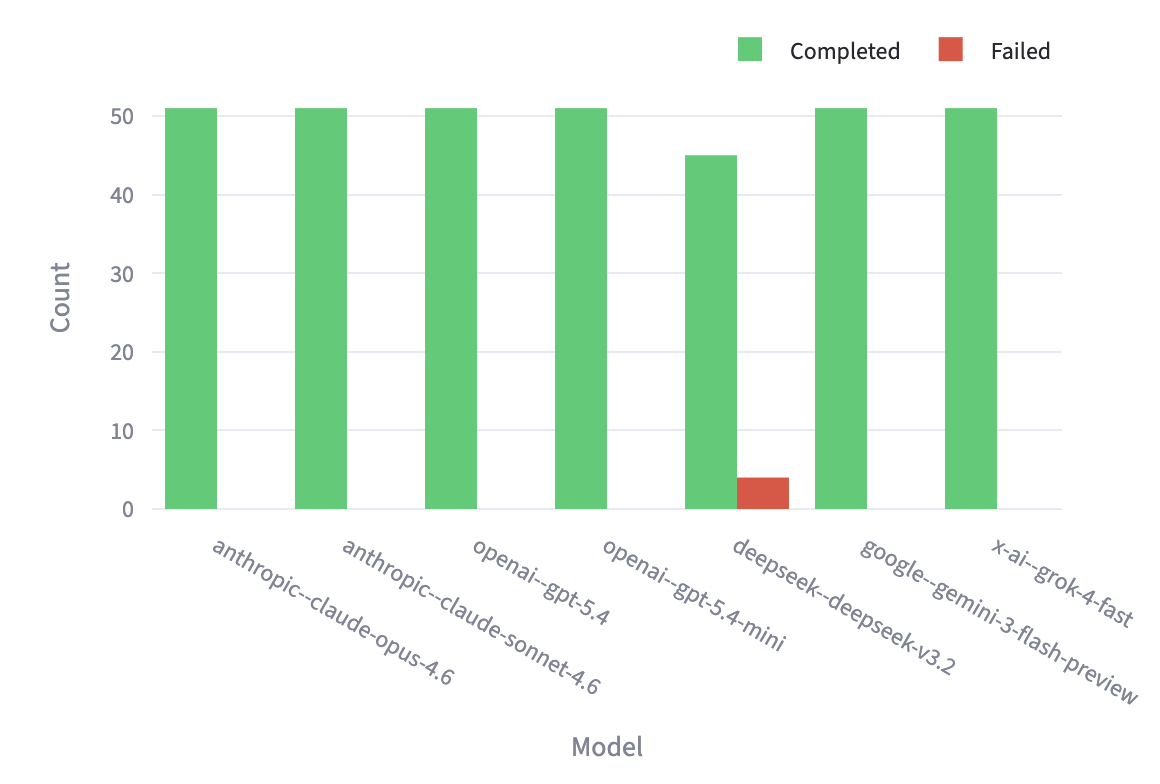
\includegraphics[width=0.9\linewidth]{figures/bench-run-status.png}
    \caption{Benchmark execution outcomes by model}
    \label{fig:bench-run-status}
\end{figure}

\subsection{Task difficulty}

Figure~\ref{fig:bench-duration-by-job} shows the mean duration of each task across all models and runs.
Individual run durations are overlaid to depict the intrinsic spread of each task.
The slowest tasks (Table~\ref{tab:hardest-tasks}) are all structural edits or large documents.
However, the fastest are narrow section-level manipulations.
The apparent $2.9$s mean for \texttt{016-large-parse-image} is an artefact of DeepSeek aborting early.
This answers question~(2): task difficulty on the suite is high for tasks involving document restructuring and repair.
The suite contains tests encompassing a distribution of easy to difficult tasks.

\begin{figure}[htb]
    \centering
    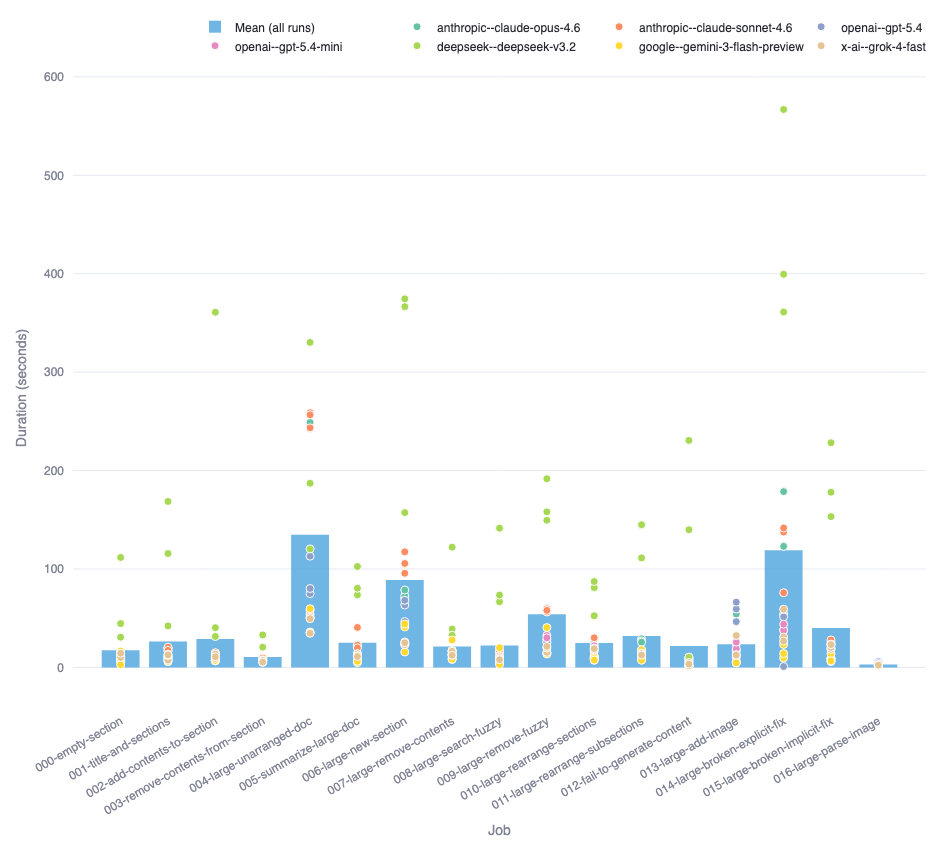
\includegraphics[width=1\linewidth]{figures/bench-duration-by-job.png}
    \caption{Run duration by benchmark task}
    \label{fig:bench-duration-by-job}
\end{figure}

\begin{table}[htb]
    \centering
    \caption{Slowest and fastest benchmark tasks}
    \label{tab:hardest-tasks}
    \begin{tabular}{lr}
        \hline
        \textbf{Task} & \textbf{Mean duration (s)} \\
        \hline
        004-large-unarranged-doc & 134.7 \\
        014-large-broken-explicit-fix & 118.9 \\
        006-large-new-section & 88.7 \\
        009-large-remove-fuzzy & 54.1 \\
        \hline
        007-large-remove-contents & 21.3 \\
        000-empty-section & 17.4 \\
        003-remove-contents-from-section & 10.6 \\
        016-large-parse-image\textsuperscript{*} & 2.9 \\
        \hline
        \multicolumn{2}{l}{\footnotesize\textsuperscript{*}~Value depressed by DeepSeek aborting the task. See Figure~\ref{fig:bench-run-status}.}
    \end{tabular}
\end{table}

\subsection{Token consumption}

Figure~\ref{fig:bench-tokens-per-model} depicts the average prompt and completion tokens per model.
The observed averages are summarised in Table~\ref{tab:token-averages}.
DeepSeek consumes approximately $64.8$K tokens per run.
This is roughly $3\times$ the volume of \texttt{gpt-5.4} on the same tasks.
This answers question~(3): a disproportionately large input average signals redundant tool use or unnecessary context retention.

\begin{figure}[htb]
    \centering
    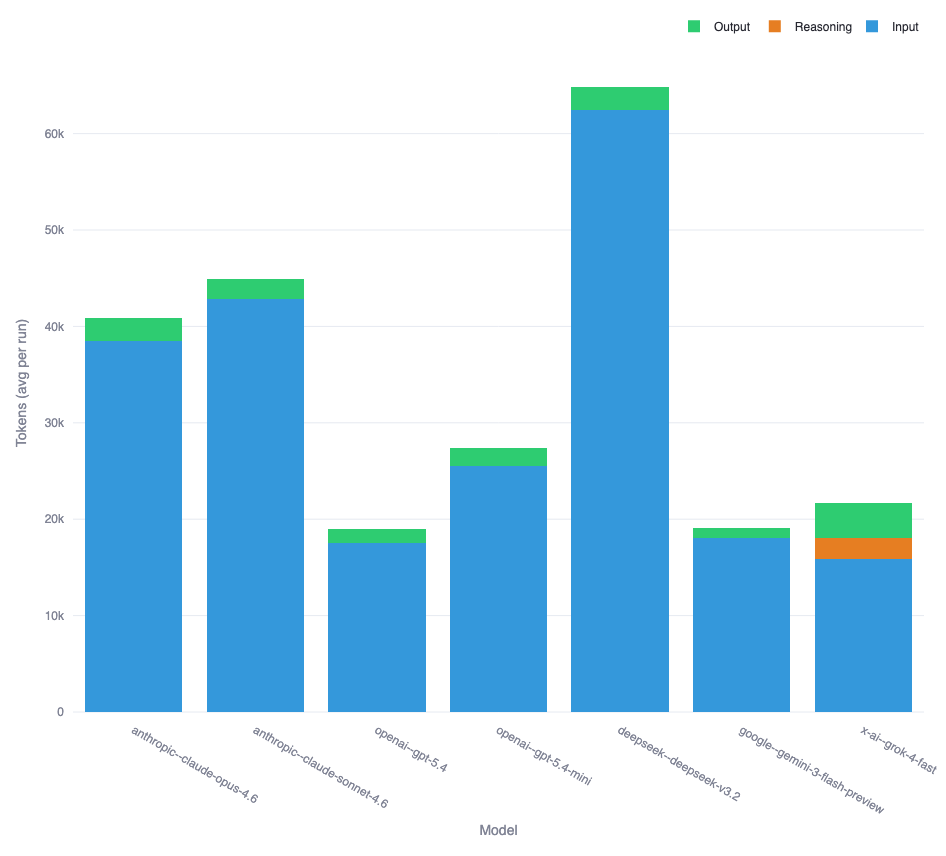
\includegraphics[width=0.9\linewidth]{figures/bench-tokens-per-model.png}
    \caption{Token usage by model and token type}
    \label{fig:bench-tokens-per-model}
\end{figure}

\begin{table}[htb]
    \centering
    \caption{Average tokens per completed run}
    \label{tab:token-averages}
    \begin{tabular}{lrr}
        \hline
        \textbf{Model} & \textbf{Input} & \textbf{Output} \\
        \hline
        \texttt{deepseek-v3.2}        & 62{,}485 & 2{,}363 \\
        \texttt{claude-sonnet-4.6}    & 42{,}854 & 2{,}084 \\
        \texttt{claude-opus-4.6}      & 38{,}503 & 2{,}327 \\
        \texttt{gpt-5.4-mini}         & 25{,}516 & 1{,}850 \\
        \texttt{grok-4-fast}          & 15{,}924 & 3{,}656 \\
        \texttt{gemini-3-flash}       & 18{,}050 & 1{,}080 \\
        \texttt{gpt-5.4}              & 17{,}511 & 1{,}507 \\
        \hline
    \end{tabular}
\end{table}

\subsection{Duration versus token volume}

Figure~\ref{fig:bench-duration-vs-tokens} plots run duration against total token count, categorised by language model.
The expected roughly linear relationship between workload size and elapsed time is present for most LLMs.
DeepSeek occupies the upper-right of the plot and is a clear outlier.
It has a mean duration of $148.6$s per run, which is much higher than the others.
This answers question~(4): the duration is predictable from token volume for six of the seven models.
DeepSeek performs poorly in this regard.

\begin{figure}[htb]
    \centering
    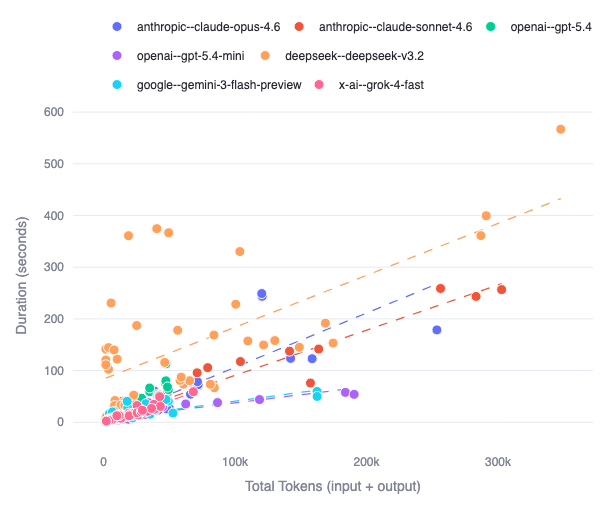
\includegraphics[width=0.9\linewidth]{figures/bench-duration-vs-tokens.png}
    \caption{Run duration compared with total token count}
    \label{fig:bench-duration-vs-tokens}
\end{figure}

\subsection{Cost per run}

Figure~\ref{fig:bench-cost-per-model} reports the mean USD cost per completed run.
Costs are computed as the sum of costs reported by the provider.
The observed ordering is given in Table~\ref{tab:cost-per-run}.
Claude~Opus is approximately $78\times$ more expensive per run than Grok~4~Fast.
As expected, the cost-efficient models outscore the flagship models at this.
However, the highest quality for a reasonable price appears to be GPT 5.4.
This answers question~(5) and frames the cost vs quality trade-off.

\begin{figure}[htb]
    \centering
    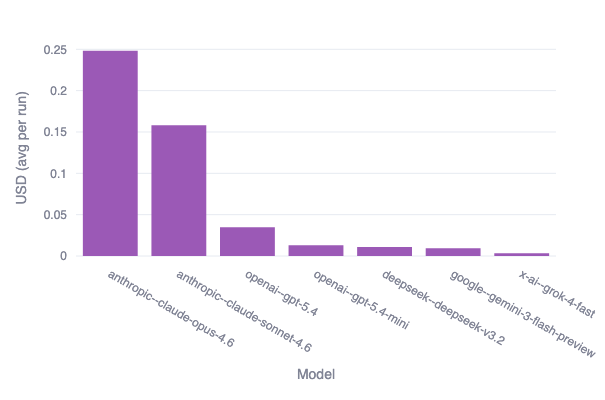
\includegraphics[width=0.9\linewidth]{figures/bench-cost-per-model.png}
    \caption{Average benchmark cost by model}
    \label{fig:bench-cost-per-model}
\end{figure}

\begin{table}[htb]
    \centering
    \caption{Mean cost per completed run}
    \label{tab:cost-per-run}
    \begin{tabular}{lrr}
        \hline
        \textbf{Model} & \textbf{Mean cost (\$/run)} & \textbf{Relative to highest} \\
        \hline
        \texttt{claude-opus-4.6}      & 0.2482 & $1.00\times$  \\
        \texttt{claude-sonnet-4.6}    & 0.1582 & $0.64\times$  \\
        \texttt{gpt-5.4}              & 0.0349 & $0.14\times$  \\
        \texttt{gpt-5.4-mini}         & 0.0130 & $0.05\times$  \\
        \texttt{deepseek-v3.2}        & 0.0108 & $0.04\times$  \\
        \texttt{gemini-3-flash}       & 0.0094 & $0.04\times$  \\
        \texttt{grok-4-fast}          & 0.0032 & $0.013\times$ \\
        \hline
    \end{tabular}
\end{table}

\subsection{Per-task model comparison}

Figure~\ref{fig:bench-duration-modelwise} projects the duration data as a bar chart grouped by task and model.
This exposes task-specific regressions that a single overall mean would conceal.
Three observations emerge:
\begin{itemize}
    \item Gemini~3~Flash is consistently the fastest endpoint across nearly every task;
    \item DeepSeek is between 3-10 times slower than the remaining models on every large-document task;
    \item The \texttt{gpt-5.4} and \texttt{gpt-5.4-mini} endpoints record very similar durations across the suite, despite \texttt{mini} consuming more input tokens on average.
\end{itemize}
This answers question~(6): the smaller models are cheaper and faster, but only marginally so.

\begin{figure}[htb]
    \centering
    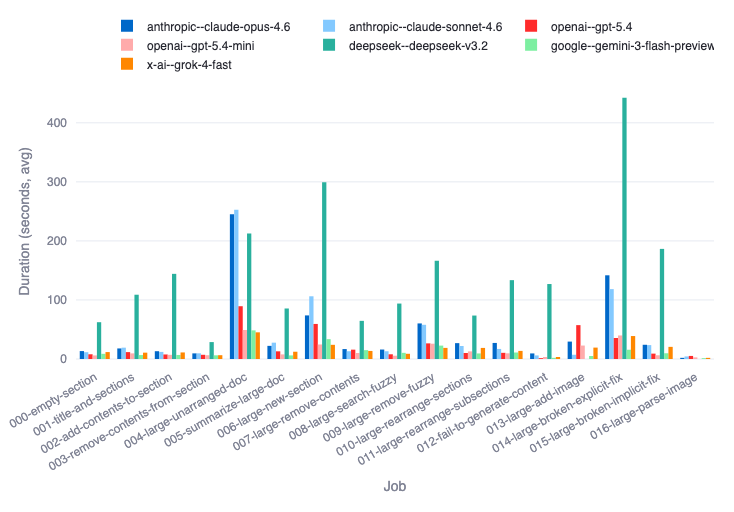
\includegraphics[width=\linewidth]{figures/bench-duration-modelwise.png}
    \caption{Task duration broken down by model}
    \label{fig:bench-duration-modelwise}
\end{figure}

\subsection{Tool invocation patterns}

The benchmark records the number of times each tool is invoked during a conversation.
Figure~\ref{fig:bench-tool-use} depicts a model-by-tool heatmap, in which each cell shows the average number of invocations of a given tool per completed run.
High invocation counts may indicate thorough exploration or inefficient looping.
The heatmap complements the scoring discussion earlier.

\begin{figure}[htb]
    \centering
    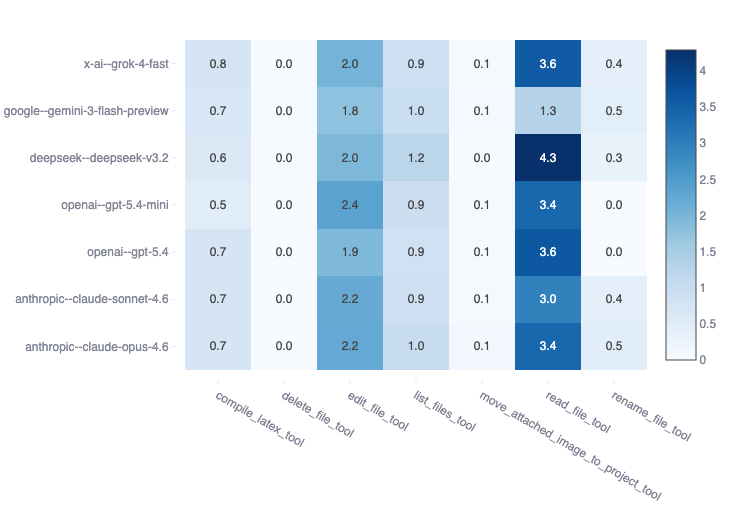
\includegraphics[width=0.9\linewidth]{figures/bench-tool-use.png}
    \caption{Tool calls by model and tool type}
    \label{fig:bench-tool-use}
\end{figure}

Three behavioural fingerprints are visible.
First, DeepSeek issues the largest number of \texttt{read\_file} invocations.
This explains the elevated input-token average reported in Table~\ref{tab:token-averages}.

Second, Gemini~3~Flash reads files comparatively little but renames them frequently
This indicates a restructure-in-place strategy that differs qualitatively from the read-then-edit pattern used by the other models.

Third, neither \texttt{gpt-5.4} nor \texttt{gpt-5.4-mini} invokes \texttt{rename\_file} at all, despite tasks for which renaming is a natural solution path.
This is a candidate for prompt- or tool-schema-level investigation in future work.
This answers question~(7): a substantial fraction of the observed cost and duration differences are due to model-specific tool usage patterns.

\subsection{Summary of findings}

Taken together, the results support the following findings.

\begin{enumerate} 
    \item All models have high task level reliability.
    Every time an error occurred it was caused by the lack of multi modal support in one of the models.

    \item The largest factor affecting task difficulty (independent of which model) is the structural edit size of the document.    
    All of the available models can perform every compatible task.

    \item There is almost two orders of magnitude difference in cost among the providers who provide the same behavior.
    The lowest cost is provided by Grok~4~Fast and Gemini~3~Flash, and the highest cost is provided by the Claude family.

    \item Tool usage patterns explain most of the observed cost and latency variance.
    DeepSeek's $5.08$ \texttt{read\_file} invocations per run is the highest of any model.
    This directly produces both its $62{,}485$ token input average and its $148.6$s mean duration.
    This is because every redundant read re-inserts file contents into the prompt on the next turn.
    Gemini~3~Flash shows the lowest \texttt{read\_file} count ($1.65$) paired with the highest \texttt{rename\_file} count ($3.83$).

    \item Significant tool-level interventions are a candidate for future work.
    The \texttt{gpt-5.4} family never invokes \texttt{rename\_file} across any of its completed runs despite several tasks admitting a rename-based solution.
    This hints at an incompatibility with GPT models and the tooling schema or a deeper issue with the model's capabilities.
\end{enumerate}

The recommended default model for the agent is \texttt{google/gemini-3-flash-preview}.
It has the lowest mean chat duration ($12.9$s) and the second-lowest mean cost ($\$0.0094$ per run).
Also, its tool-use strategy aligns well with the large-scale editing tasks in the benchmark.

\texttt{x-ai/grok-4-fast} is a credible secondary choice where cost is the overriding concern.
At $\$0.0032$ per run it is roughly $3\times$ cheaper again.
However, its slightly longer mean duration ($16.4$s) makes it marginally less suited to an interactive chat experience.

The Anthropic models are between one and two orders of magnitude more expensive per run than these two alternatives.
They cannot be justified for this workload based on efficiency metrics.
This may change if the models outperform the others on a quality metric.

DeepSeek~v3.2 is not recommended in any configuration.
It is missing multimodal support and its redundant read behaviour is not efficient.
